% Created 2024-02-15 Thu 18:31
% Intended LaTeX compiler: pdflatex
\documentclass[11pt]{article}
\usepackage[utf8]{inputenc}
\usepackage[T1]{fontenc}
\usepackage{graphicx}
\usepackage{longtable}
\usepackage{wrapfig}
\usepackage{rotating}
\usepackage[normalem]{ulem}
\usepackage{amsmath}
\usepackage{amssymb}
\usepackage{capt-of}
\usepackage{hyperref}
\usepackage[margin=2cm]{geometry}
\author{Ian Grant}
\date{\today}
\title{Lab 1, Spatial Data Analysis}
\hypersetup{
 pdfauthor={Ian Grant},
 pdftitle={Lab 1, Spatial Data Analysis},
 pdfkeywords={},
 pdfsubject={},
 pdfcreator={Emacs 29.0.92 (Org mode 9.6.6)}, 
 pdflang={English}}
\makeatletter
\newcommand{\citeprocitem}[2]{\hyper@linkstart{cite}{citeproc_bib_item_#1}#2\hyper@linkend}
\makeatother

\usepackage[notquote]{hanging}
\begin{document}

\maketitle

\section{Boxplots}
\label{sec:org1e53fc9}
The boxplots in the screenshots shown below show the distribution of rent in 2008. The maps show the distribution of household size. In the first image, selecting lower Manhattan reveals that this group of sub-boroughs has low household size (highlighted on the map) and high rent (highlighted in the boxplot, on the right side). In the second image, selecting two sub-boroughs in northern Manhattan and the Bronx shows that while both have very low rent (highlighted in the boxplot), they diverge sharply in household size.

\begin{center}
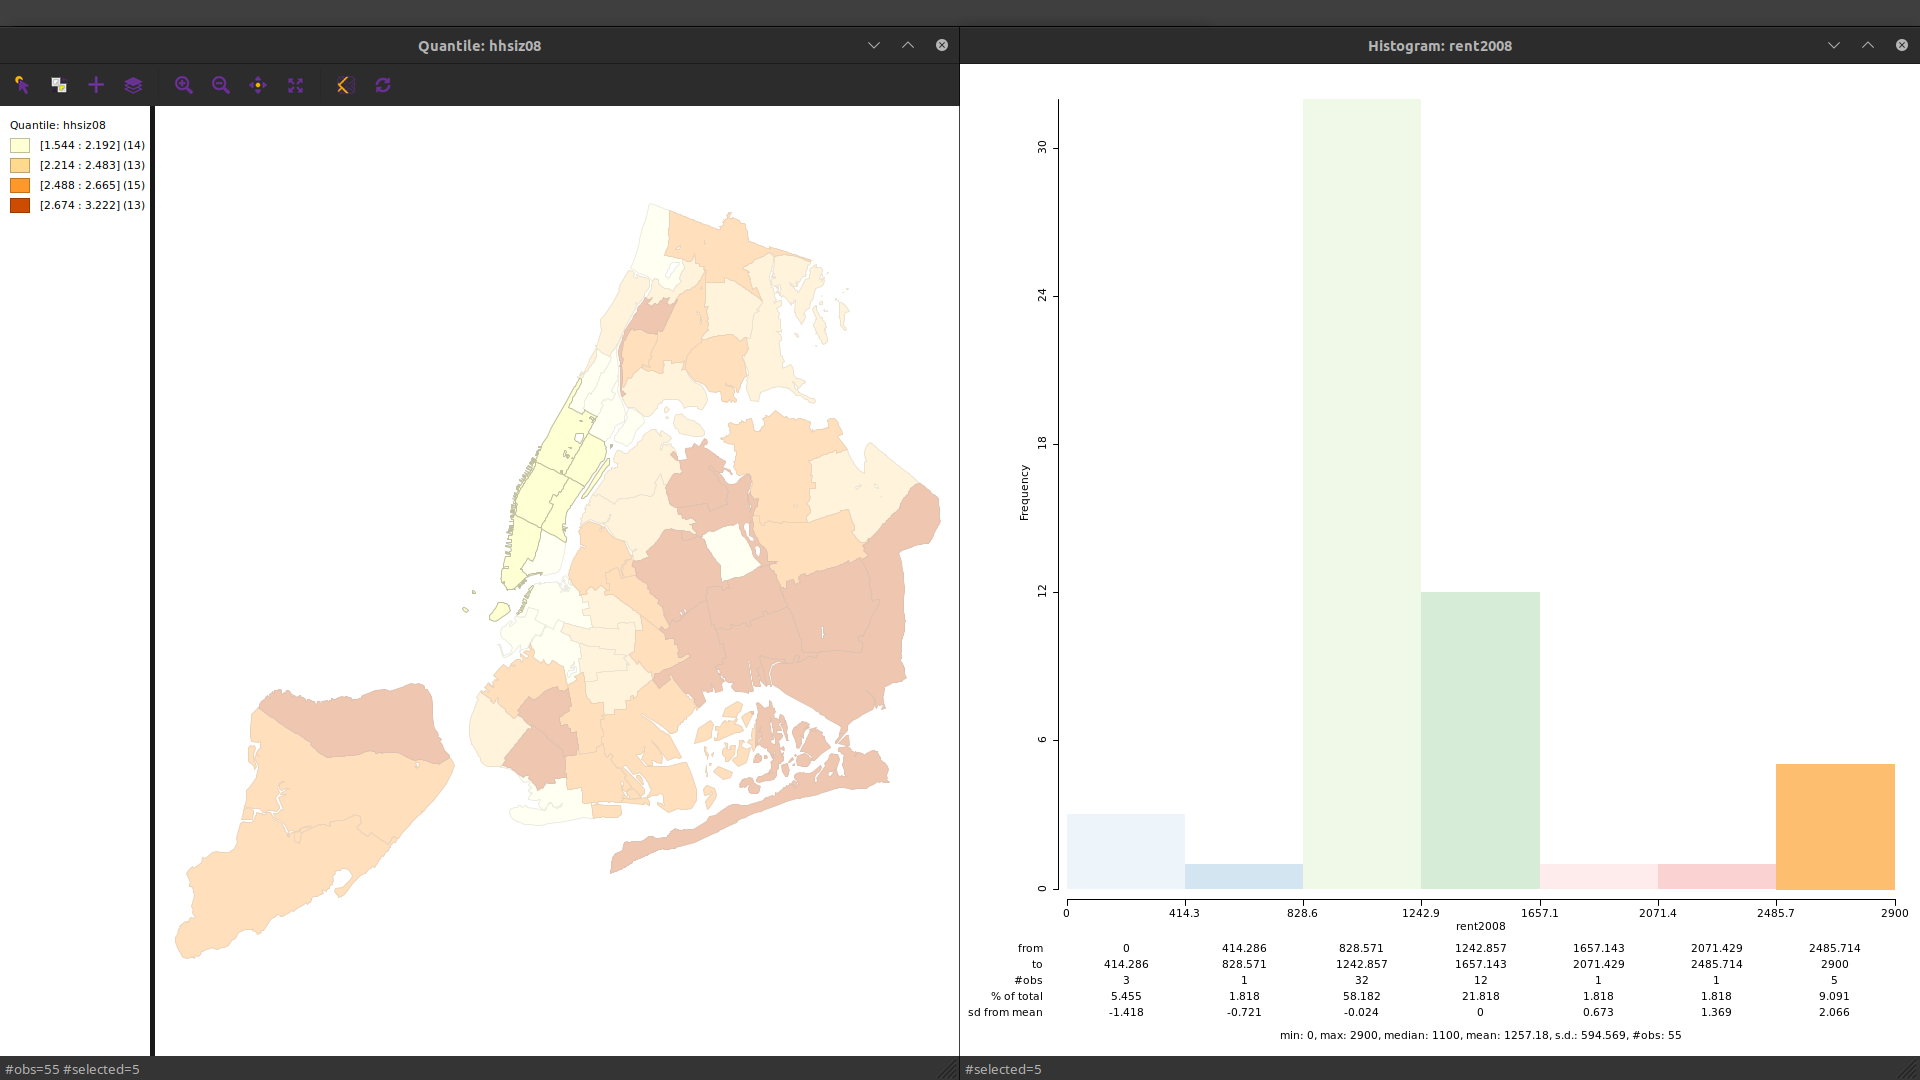
\includegraphics[width=.9\linewidth]{hist_hhsize_high.png}
\end{center}
\begin{center}
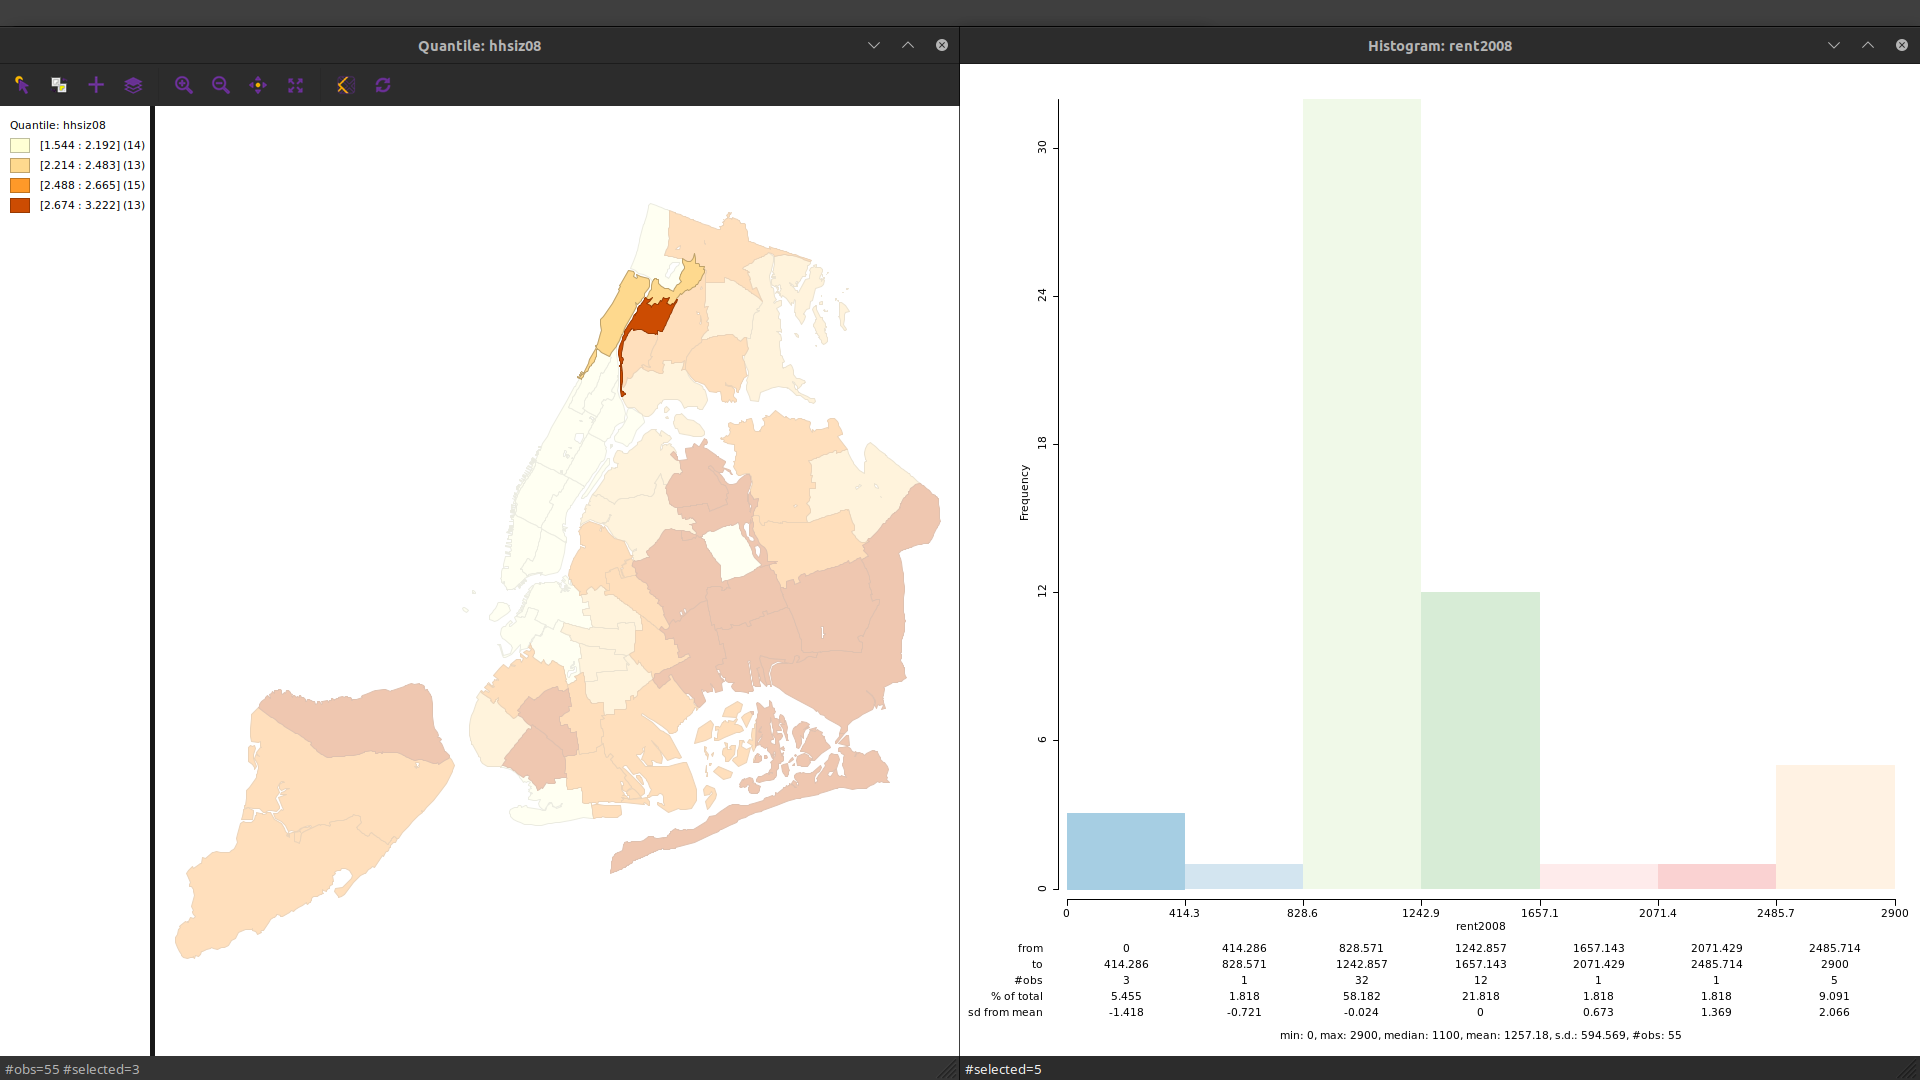
\includegraphics[width=.9\linewidth]{hist_hhsize_low.png}
\end{center}

\section{Scatterplots}
\label{sec:orgf5011b8}
We can using a scatterplot and the accompanying regression to characterize how rent changed from 2005 to 2008. The scatterplot shown below shows that rent increases were relatively uniform with the exception of a sub-borough in the South Bronx which is an outlier, highlighted in the map below.

\begin{center}
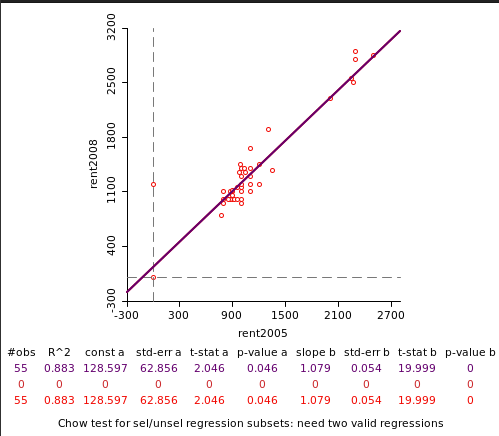
\includegraphics[width=.9\linewidth]{scatter.png}
\end{center}
\begin{center}
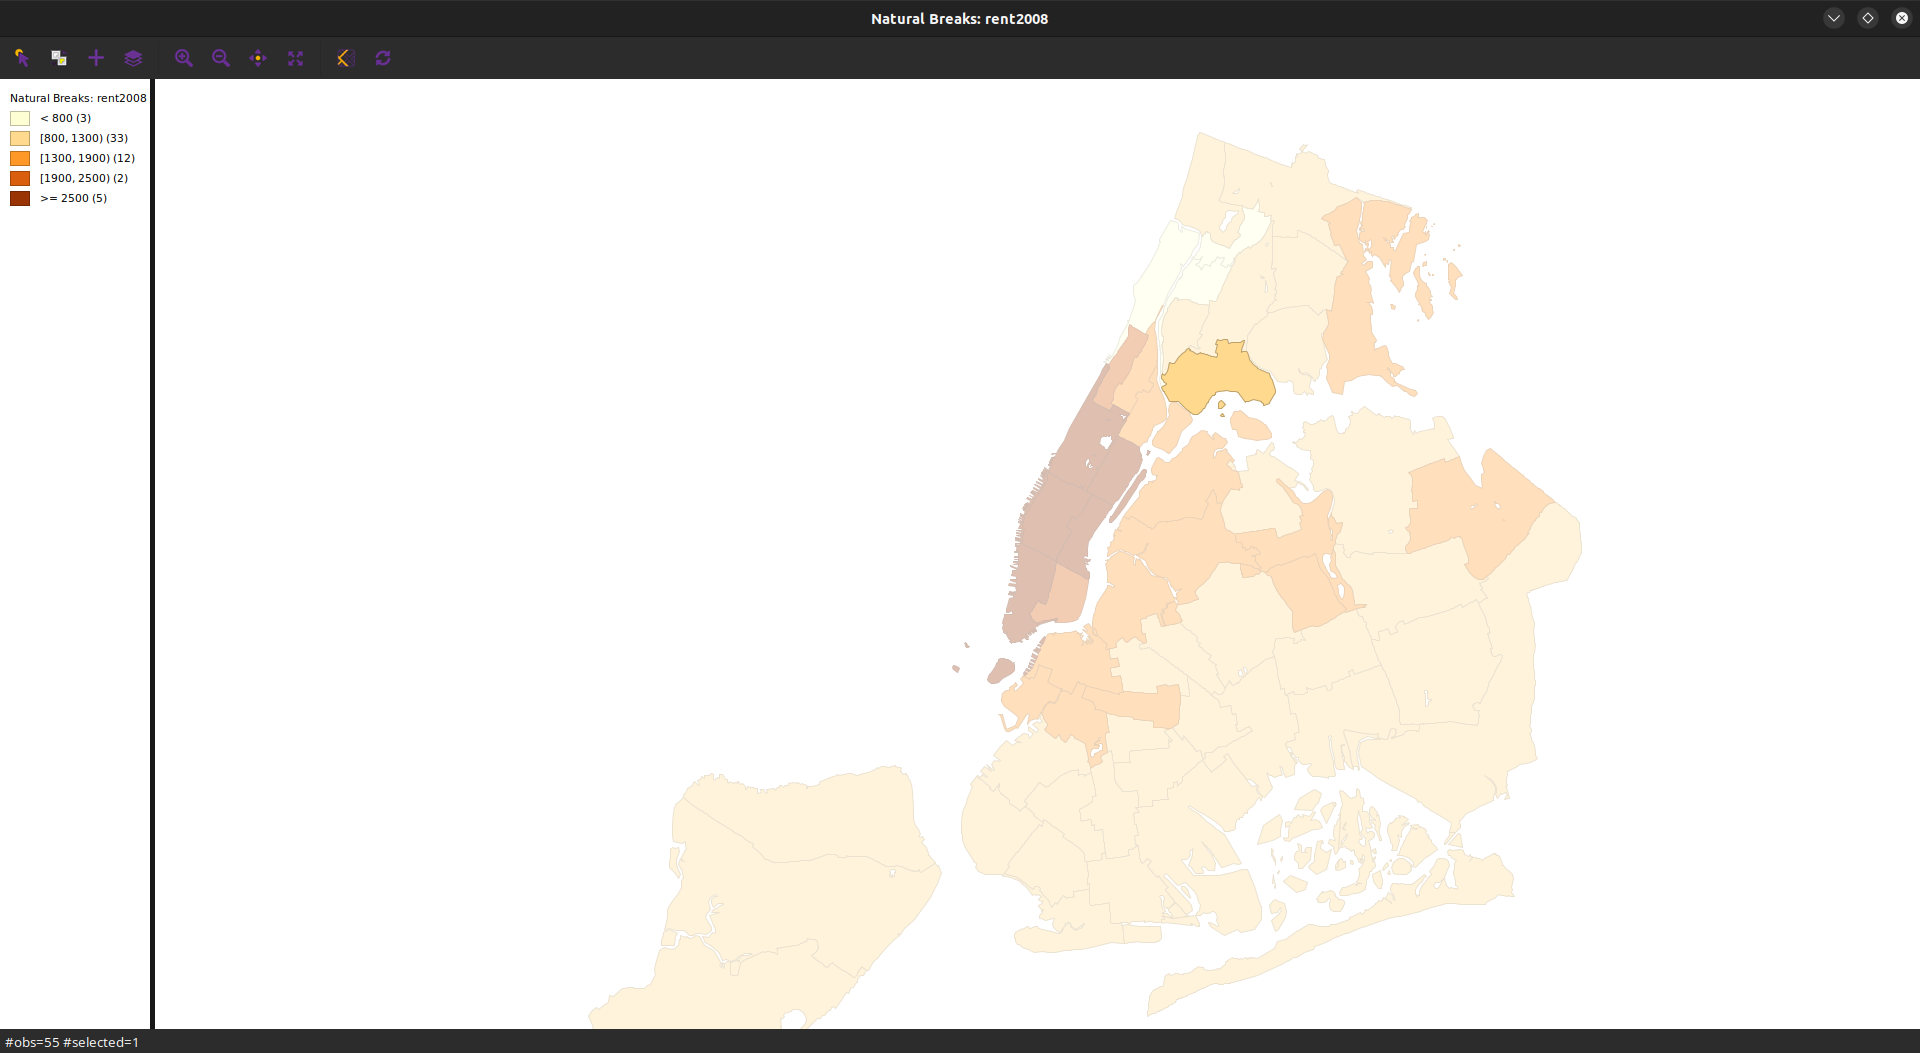
\includegraphics[width=.9\linewidth]{outlier.png}
\end{center}

Because this outlier is on the extreme low end of the 2005 rent
distribution, we can expect it to have an outsize impact on the
regression fit. Indeed, if we exclude the outlier from the regression,
the R squared increases from .883 to .949 (below). Also, the intercept
decreases from \$128.60 to \$17.768 and its p-value becomes
non-significant. An intercept indistinguishable from zero makes sense
if we expect rent increases to occur as a factor of existing rent, not
as a fixed increase regardless of current rent. Since the slope of the
new regression is 1.164 and the intercept is near zero, we can
conclude that the sub-boroughs' median rent increased by an average of
about 16.5\% over the three-year period from 2005 to 2008.

\begin{center}
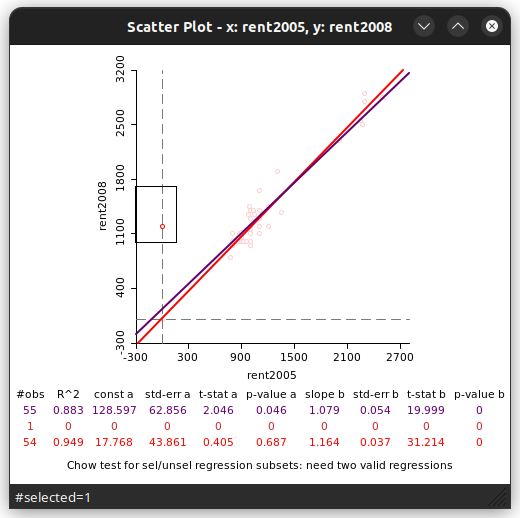
\includegraphics[width=.9\linewidth]{scatter_excluding_outlier.png}
\end{center}

Finally, we can ask whether some geographical areas experienced different patterns of rent increase. Let's look at lower Manhattan, which has the city's highest rents. Selecting just these sub-boroughs, shown at the top right of the scatterplot below, produces slightly different slopes. But the Chow test for a difference in slopes produces a non-significant p-value of .252; we cannot conclude that Manhattan's rent-increase trend is different from the rest of the city's.

\begin{center}
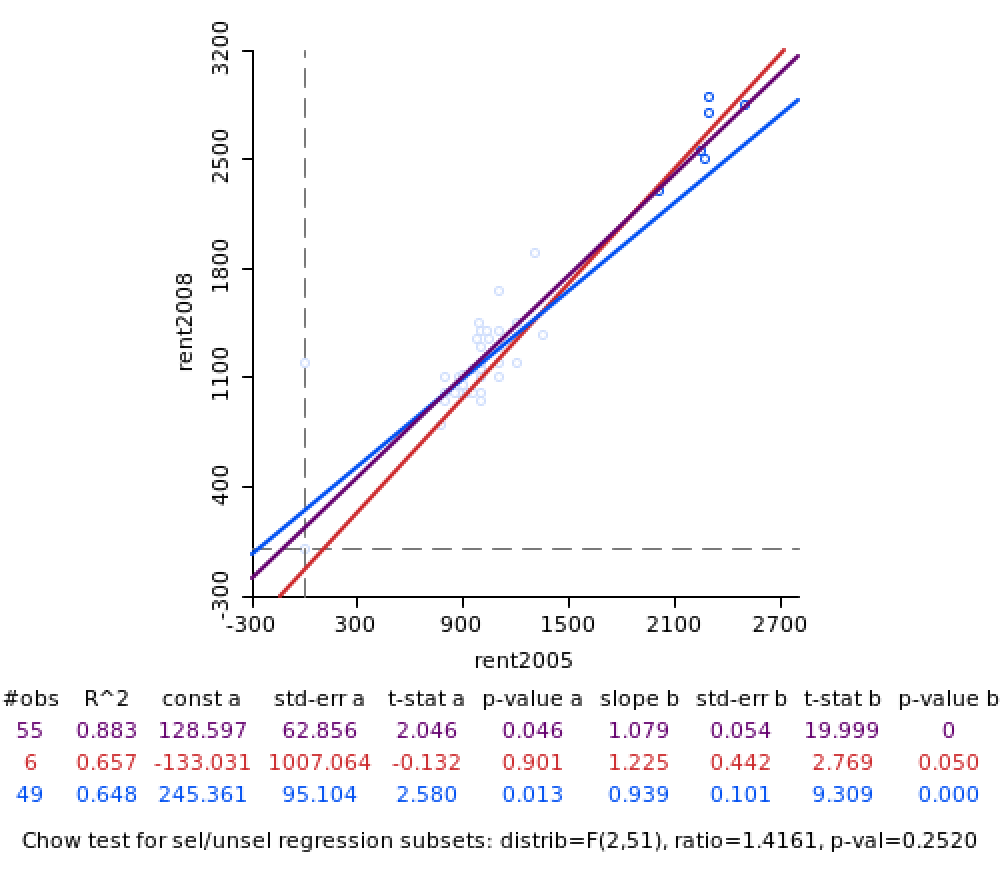
\includegraphics[width=.9\linewidth]{scatter_lower_manhattan.png}
\end{center}

\section{Bubble plot}
\label{sec:org31096f8}
This same group of rich sub-boroughs in lower Manhattan stands out on a bubble plot of percent public assistance and percent children. The sub-boroughs are shown on the lower left of the plot, with the lowest percentage of children and the lowest percent on public assistance. Meanwhile, the size and shape of the bubble shows that rent tracks closely with these two variables, with the highest-rent sub-boroughs (lower Manhattan) also having the lowest values for children and public assistance.

\begin{center}
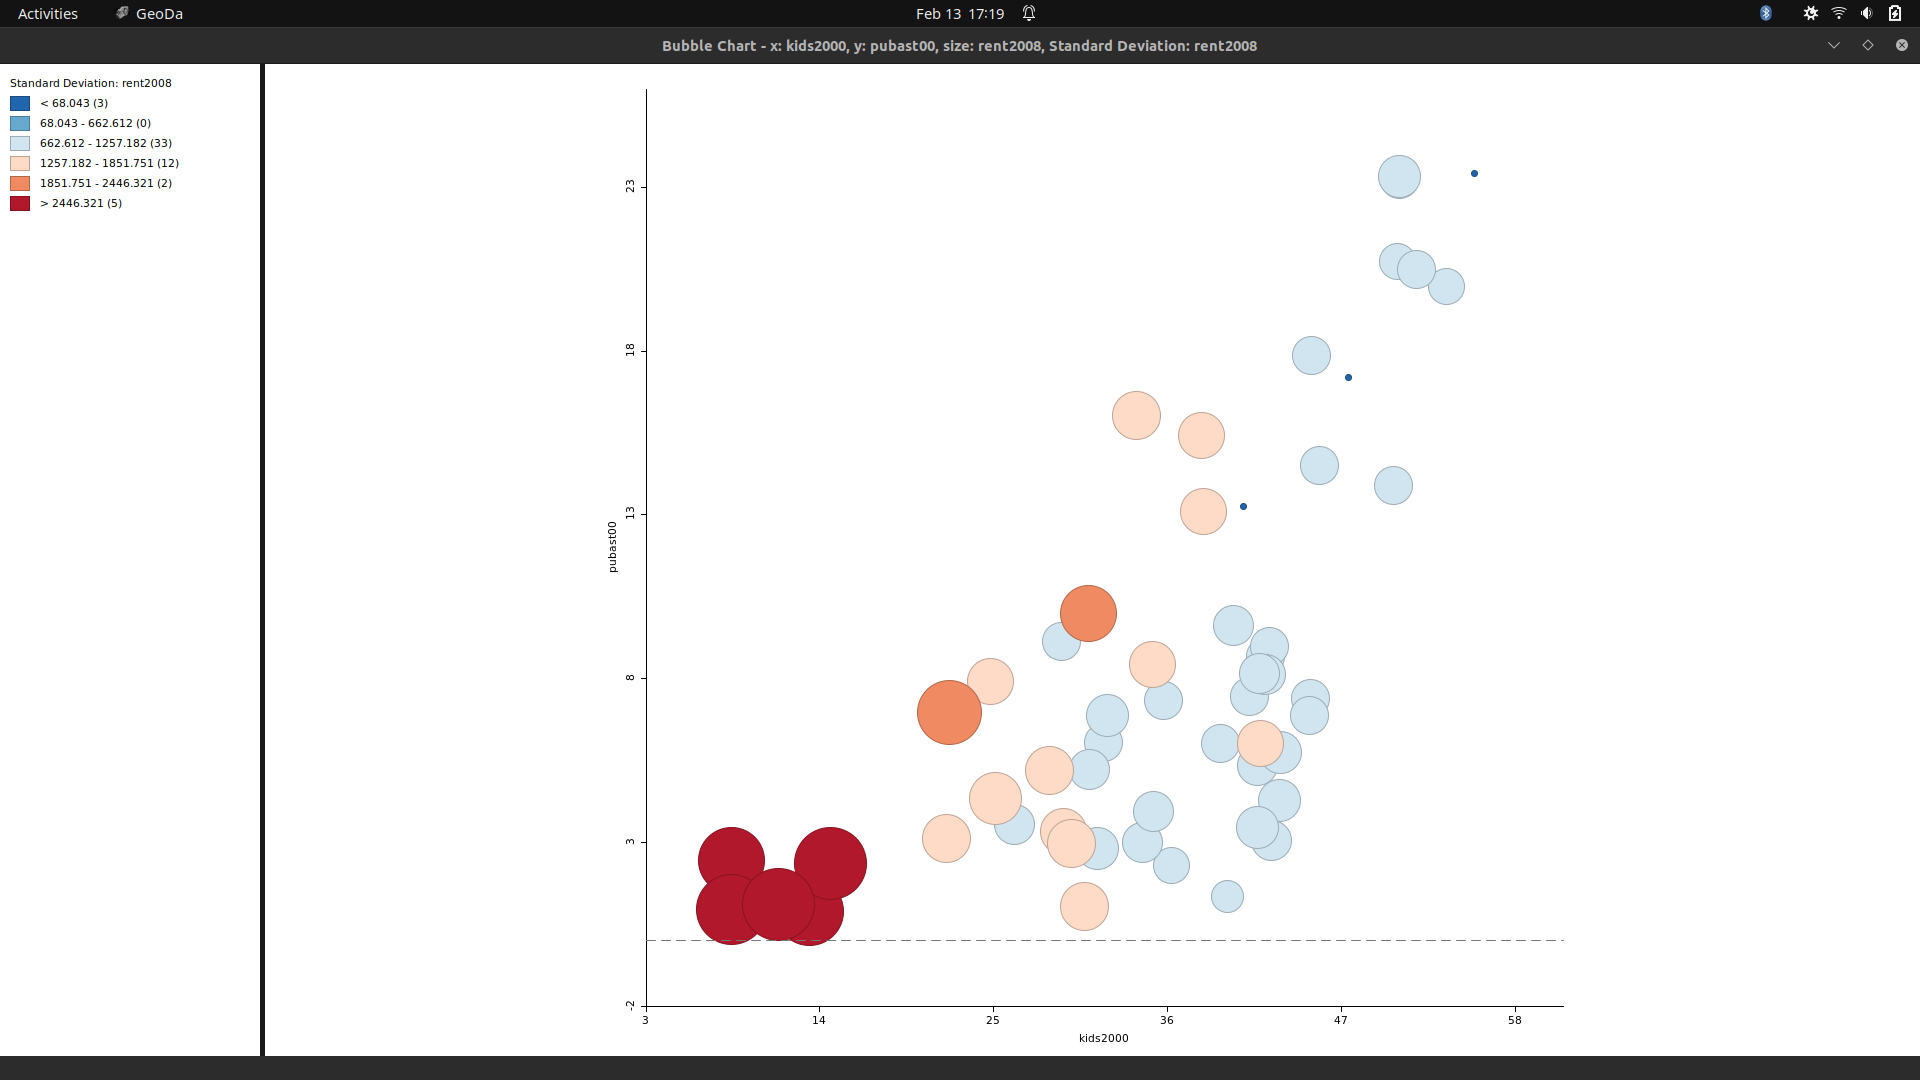
\includegraphics[width=.9\linewidth]{bubble.png}
\end{center}

\section{3D scatter plot}
\label{sec:orgc58ca5a}
These outlying lower and midtown Manhattan sub-boroughs are even clearer in a 3D scatterplot. In the screenshot below, the sub-boroughs are shown in dark red on the map and in yellow in the 3D scatterplot. Their placement in the 3D plot indicates that they have lower percent public assistance, high rent, and low household size.

\begin{center}
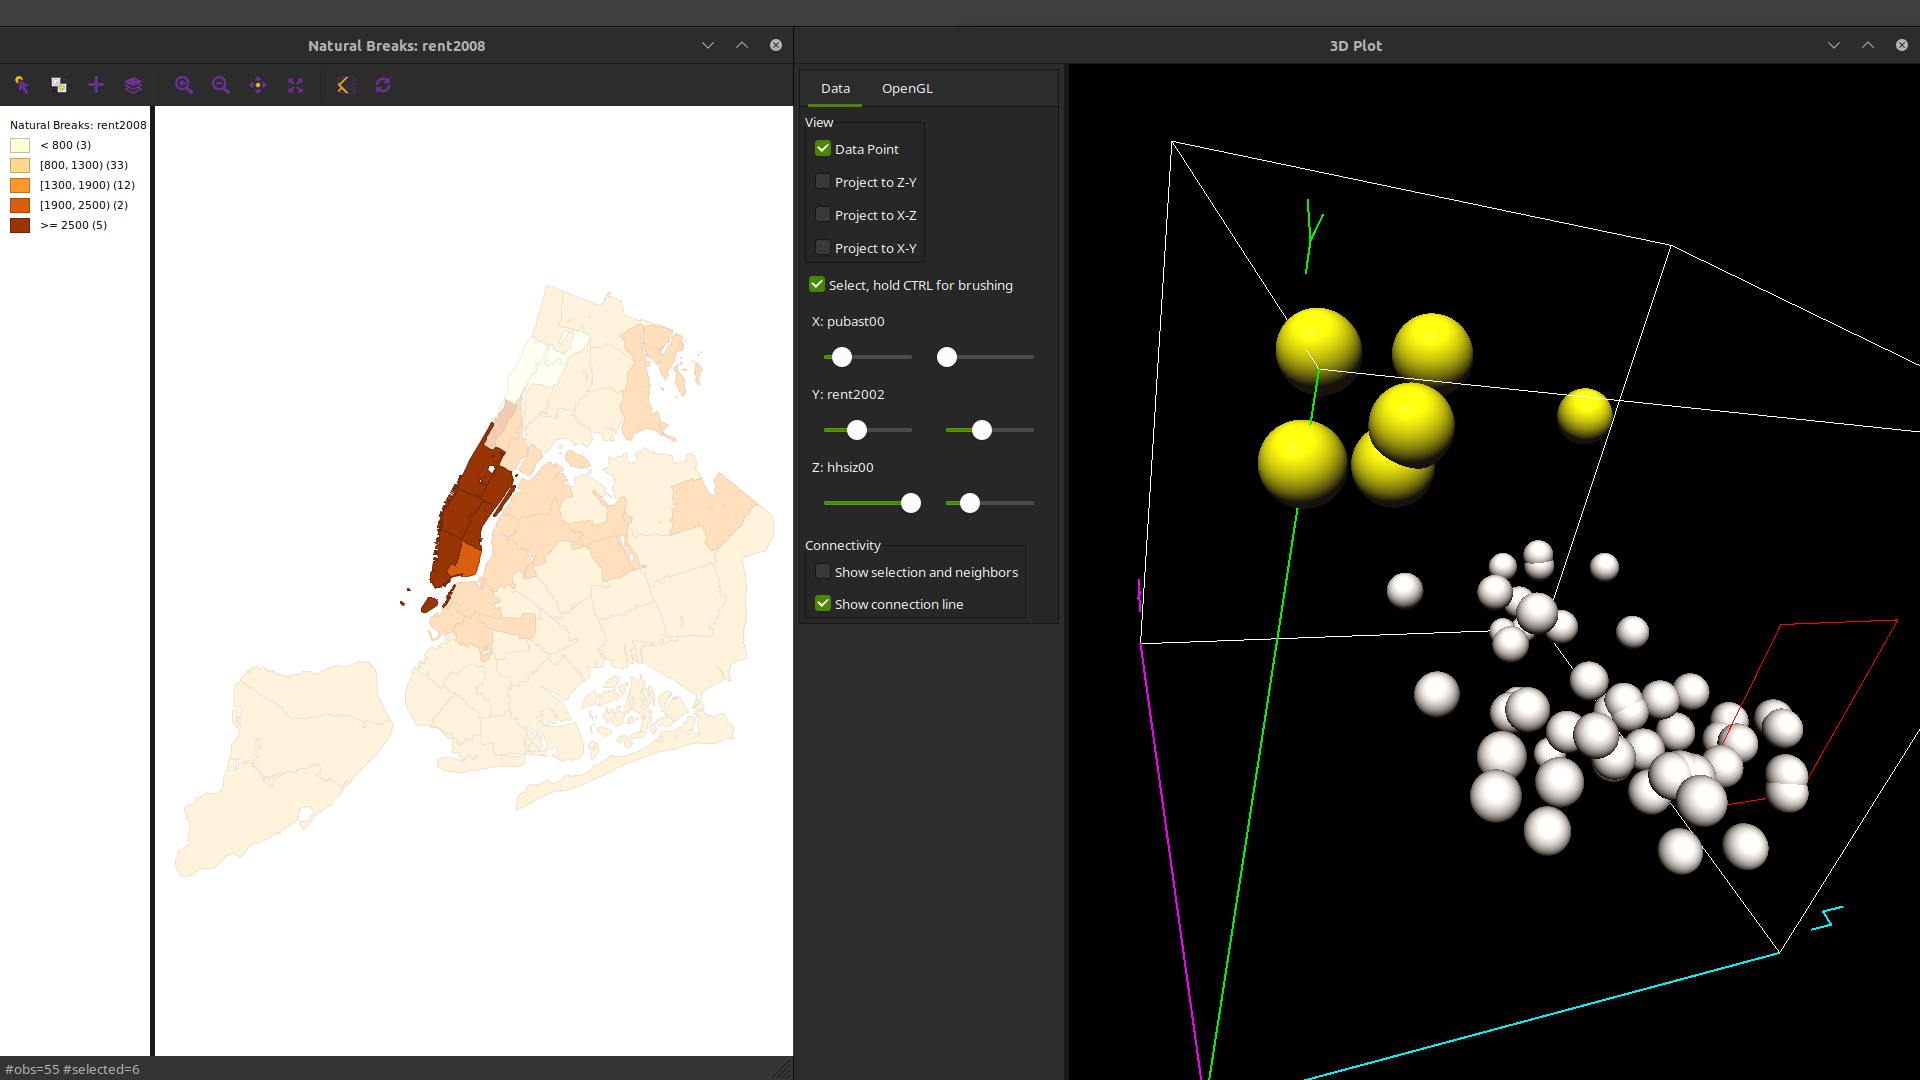
\includegraphics[width=.9\linewidth]{3d_scatter_lower_manhattan.png}
\end{center}

\section{Parallel coordinates plot}
\label{sec:orgb61433c}
A similar picture emerges with the parallel coordinate plot. Across rent, percent of housing stock that is rental units, percent of population on public assistance, percent children, and household size, the rich boroughs of lower and midtown Manhattan follow a similar trajectory, with high rent, medium percent housing stock, and low values for the other variables.

\begin{center}
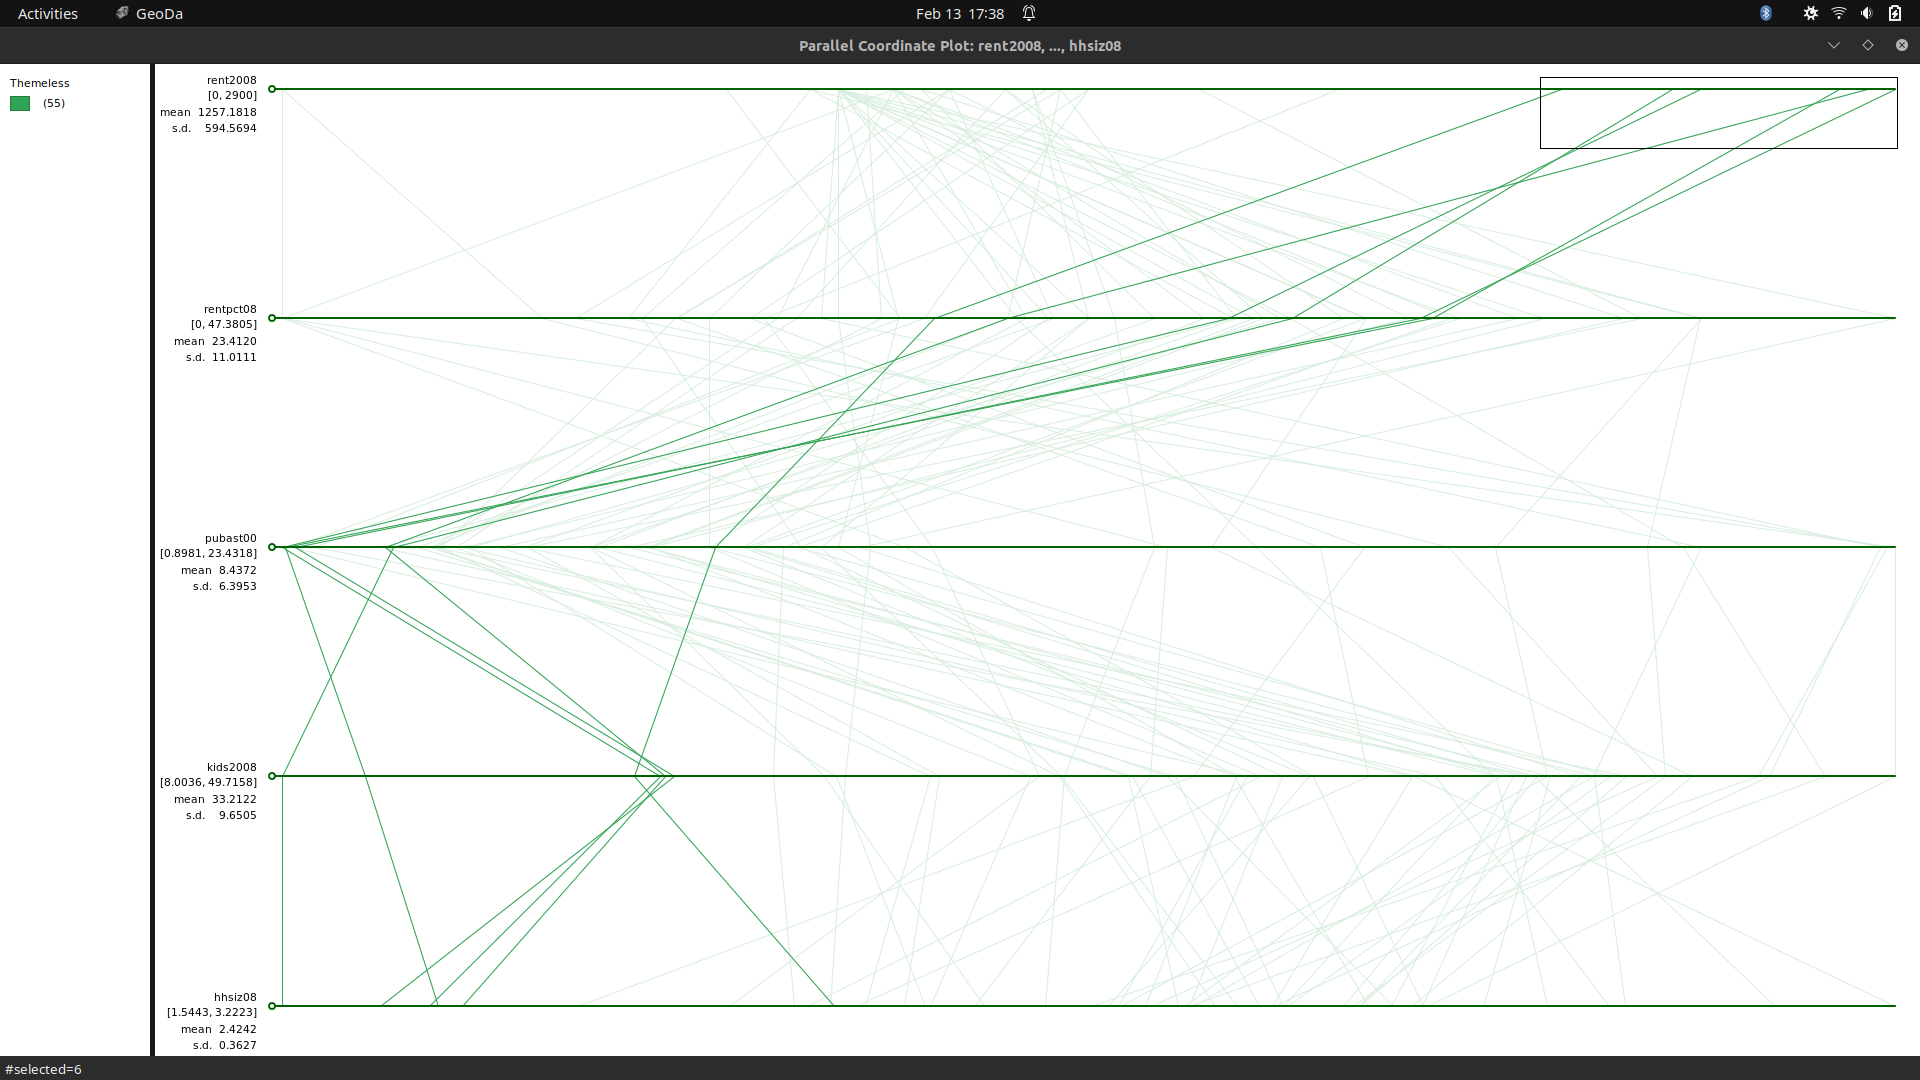
\includegraphics[width=.9\linewidth]{parallel_coord.png}
\end{center}

\section{Conditional scatterplot}
\label{sec:org4a7c5e1}
\begin{center}
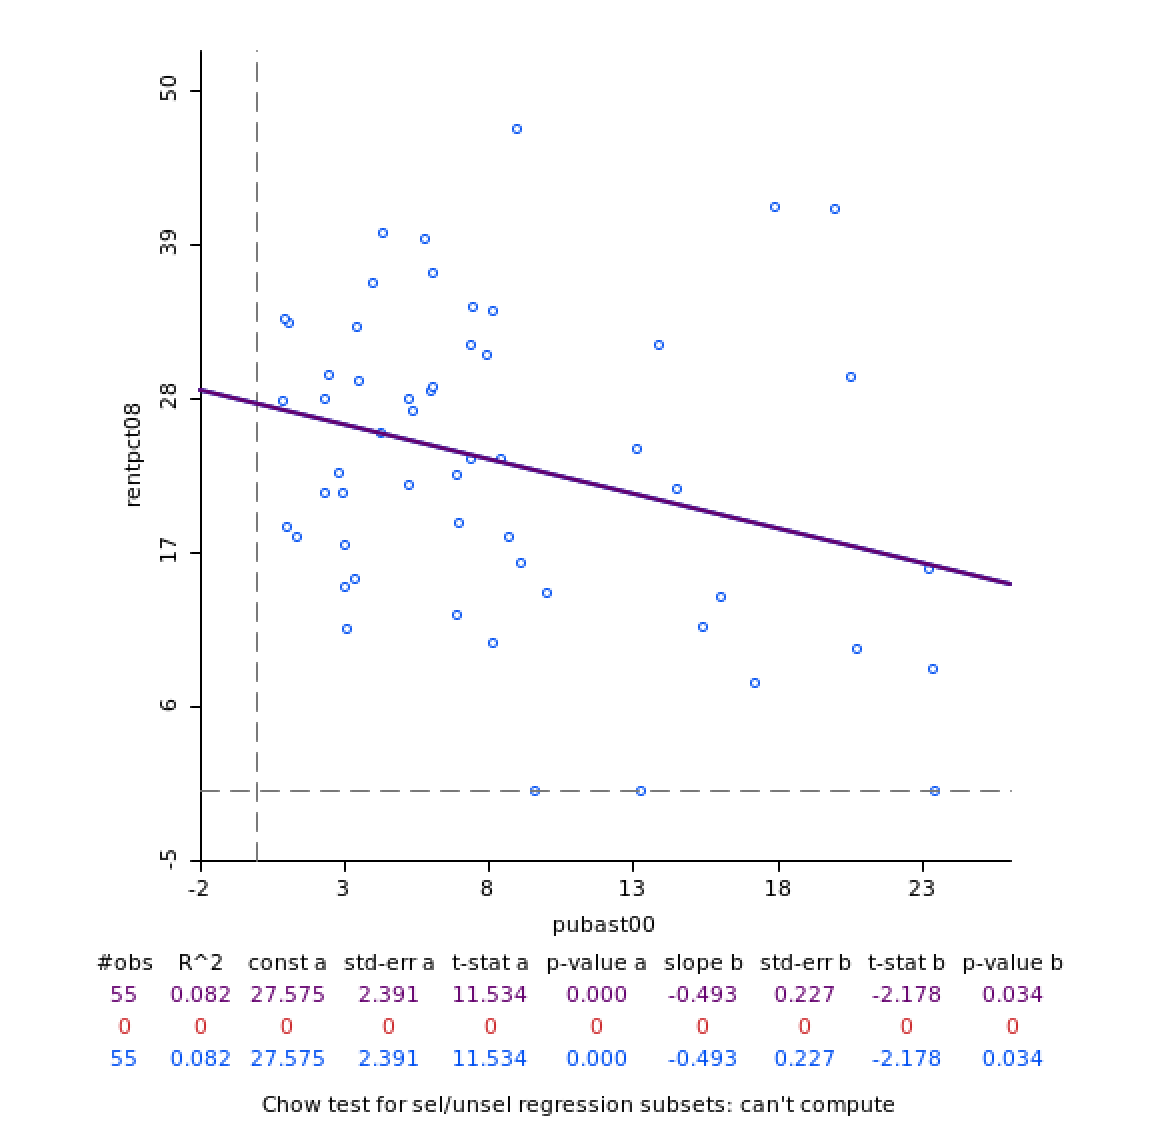
\includegraphics[width=.9\linewidth]{rent_pub_ast_scatter.png}
\end{center}

Overall, rent in 2008 shows a significant but weak relationship with public assistance in 2000 (the most recent available data in the dataset; scatterplot shown above). However, there is a lot of variation around the trend line and the R squared value of this fit is .082. A conditional scatterplot may help to clarify the relationship.

Below, the same scatterplot is reproduced with children in 2008 and
household size in 2008 as conditions. Now we can see that there is a
strong negative relationship between 2008 rent and 2000 public assistance for sub-boroughs with fewer children and smaller households (bottom left). By selecting the points in this sub-plot, we can see that they are mostly relatively central neighborhoods of the city in Manhattan and western Brooklyn and Queens, though there are some Bronx and eastern Queens sub-boroughs included as well.

\begin{center}
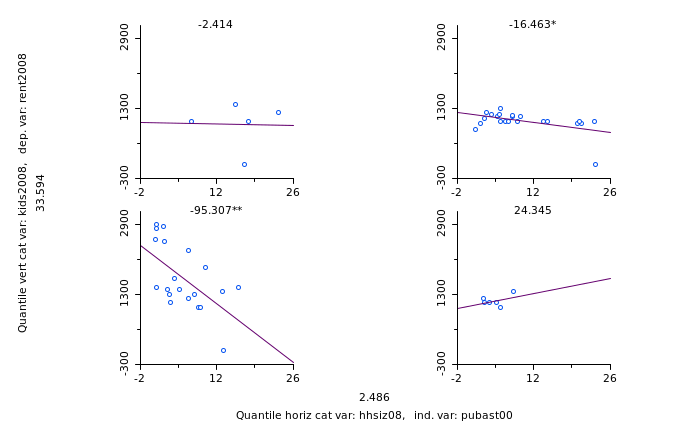
\includegraphics[width=.9\linewidth]{conditional_scatter.png}
\end{center}
\begin{center}
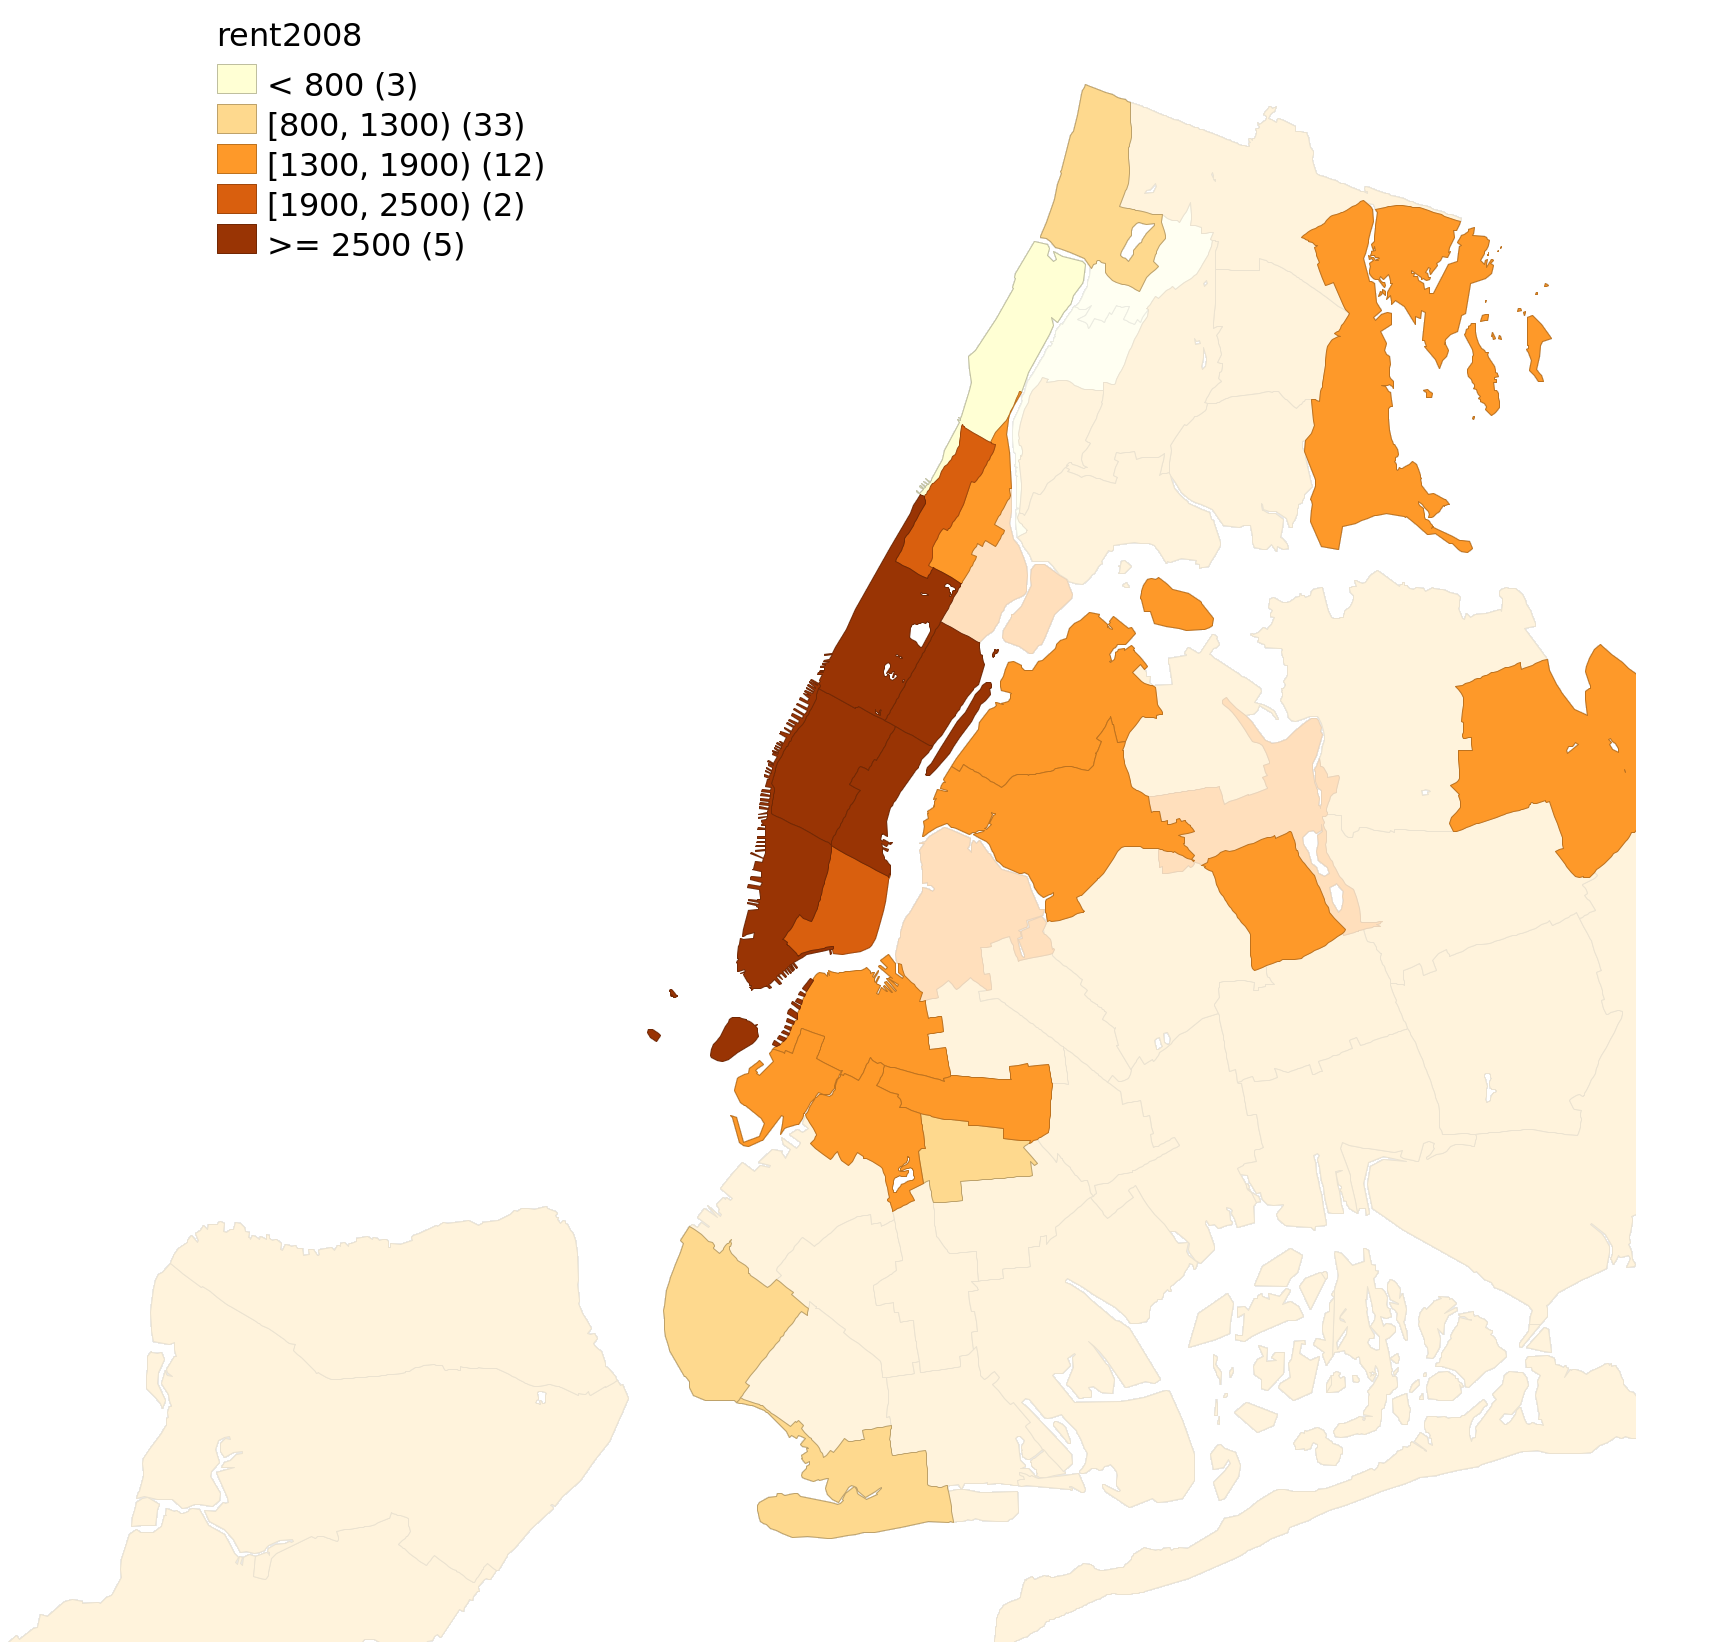
\includegraphics[width=.9\linewidth]{map_conditional_scatter.png}
\end{center}
\end{document}